% ------------------------------------------------------------------------ %
% !TEX encoding = UTF-8 Unicode
% !TEX TS-program = pdflatex
% !TEX root = ../Tesi.tex
% !TEX spellcheck = it-IT
% ------------------------------------------------------------------------ %
%
% ------------------------------------------------------------------------ %
% 	NOME CAPITOLO
% ------------------------------------------------------------------------ %
%
\chapter{BlueSentinel: the Occupancy Monitoring System}
\chaptermark{The BlueSentinel System}
%\markboth{The BlueSentinel System}{The BlueSentinel System}	% headings
%
\label{cap:bluesentinel}
%
\section{Intro}
\lipsum[5]

\section{Choosing the Enabling Technology}
\label{sec:technology}
In the {\hyperref[cap:soa]{previous chapter}}, many possible technological solutions to build indoor location monitoring systems have been reviewed. During the preliminary analysis of our work, all the available technologies have been considered in order to satisfy the occupancy monitoring requirements and a feasible solution for both users and infrastructures.

Considering the comparison summarized in table \ref{tab:od_soa}, it can be deduced that the only solutions able to guarantee a true real-time detection of users are cameras and wireless based solutions. When comparing this two approaches, cameras revealed to have many more drawbacks with respect to wireless solutions.
Camera based systems require a high computational effort to perform real-time body recognition on indoor video (or images) streams. The compute-intensive peculiarity makes the approach not suitable to scale up for large buildings, with tens or thousand rooms and users.
Wireless based solutions tend to provide easily an outcome in real-time, or with a tolerable delay. Raw data produced by wireless systems is usually far more lightweight to process (for example compared to images), making the solution attractive for large indoor areas.

Inside the wireless scope, the choice is restricted to technologies that all users have already available in their mobile devices, so to avoid the employment of additional objects. The first one is certainly WiFi. WiFi based localization solutions have been deeply investigated, also because of WiFi infrastructure is already present in almost all buildings. However, for monitoring purposes, they are not able to provide real-time location data for long execution periods. This issue is explained in detail in section \ref{subsec:wips_od} and summarized here. There exist two ways to localize a mobile device using WiFi connectivity, an \emph{active} and a \emph{passive} method. The active method requires an application installed on mobile device that keeps an active connection with all the surrounding hotspots, and continuously notify collected data using an Internet connection. However, battery consumption related to WiFi operations is too high to reach many hours of execution. The passive method instead doesn't require any installed application on mobile device, but simply exploits WiFi packets sent from devices during their usual activity. Unfortunately, using this approach, is nearly impossible to obtain real-time detection since mobile operating systems apply aggressive sleep policies to WiFi module in order to limit consumptions. A WiFi connected smartphone during sleep can spend several minutes without emits any signal, making the system unresponsive to users movements \cite{Balaji2013}.

The remaining available wireless technology is Bluetooth, and in particular Bluetooth Low Energy. Since 2010, BLE chips (able to work with classic and Low Energy enabled Bluetooth) have been built into in an increasing number of smartphones, tablets or wearables (as instance, Apple has incorporated them in its products since the iPhone 4S in 2011).
Devices using BLE consume ten times less then WiFi and a fraction of the power of classic Bluetooth \cite{Choperena2013}.
However, at the best of our knowledge, BLE has been employed for localization only through passive appliances (like beacons) that leave the burden on the mobile device, forcing it to run positioning algorithms continuously and notify the result through energy-hungry connectivities.
In order to fully exploit energy efficiency of BLE, the proposed system relies on BLE mobile advertisement (section \ref{sec:advertisement}), a particular BLE signal transmission compatible with almost all mobile devices since few years.
%With the diffusion in the last few years of devices enabled with peripheral mode BLE chipset, BLE advertisement becomes possible on mobile devices
%This makes BLE an excellent technology for a real-time positioning solution.


\section{Mobile BLE advertisement}
\label{sec:advertisement}
As explained in section \ref{subsec:BLEprotocol}, BLE specification divides Bluetooth devices in two classes: \emph{Central} and \emph{Peripheral} devices (figure \ref{fig:cent-per}). Peripheral devices generates data, like sensor readings or audio streams, while Central devices consumes it. This BLE specification was intended to classify smartphones and PC as centrals, while accessories as peripherals.

BLE has also two ways of communicating. The first way is establishing a \emph{Connection} between a peripheral and a central device. Every connection however, requires a preliminary pairing phase between the two devices. This makes unfeasible the employment of BLE connections in monitoring applications, since a mobile device (central) would be forced to perform a pairing with every single reference node (peripheral) before monitoring can start.

\begin{figure}[h!tb]
\centering
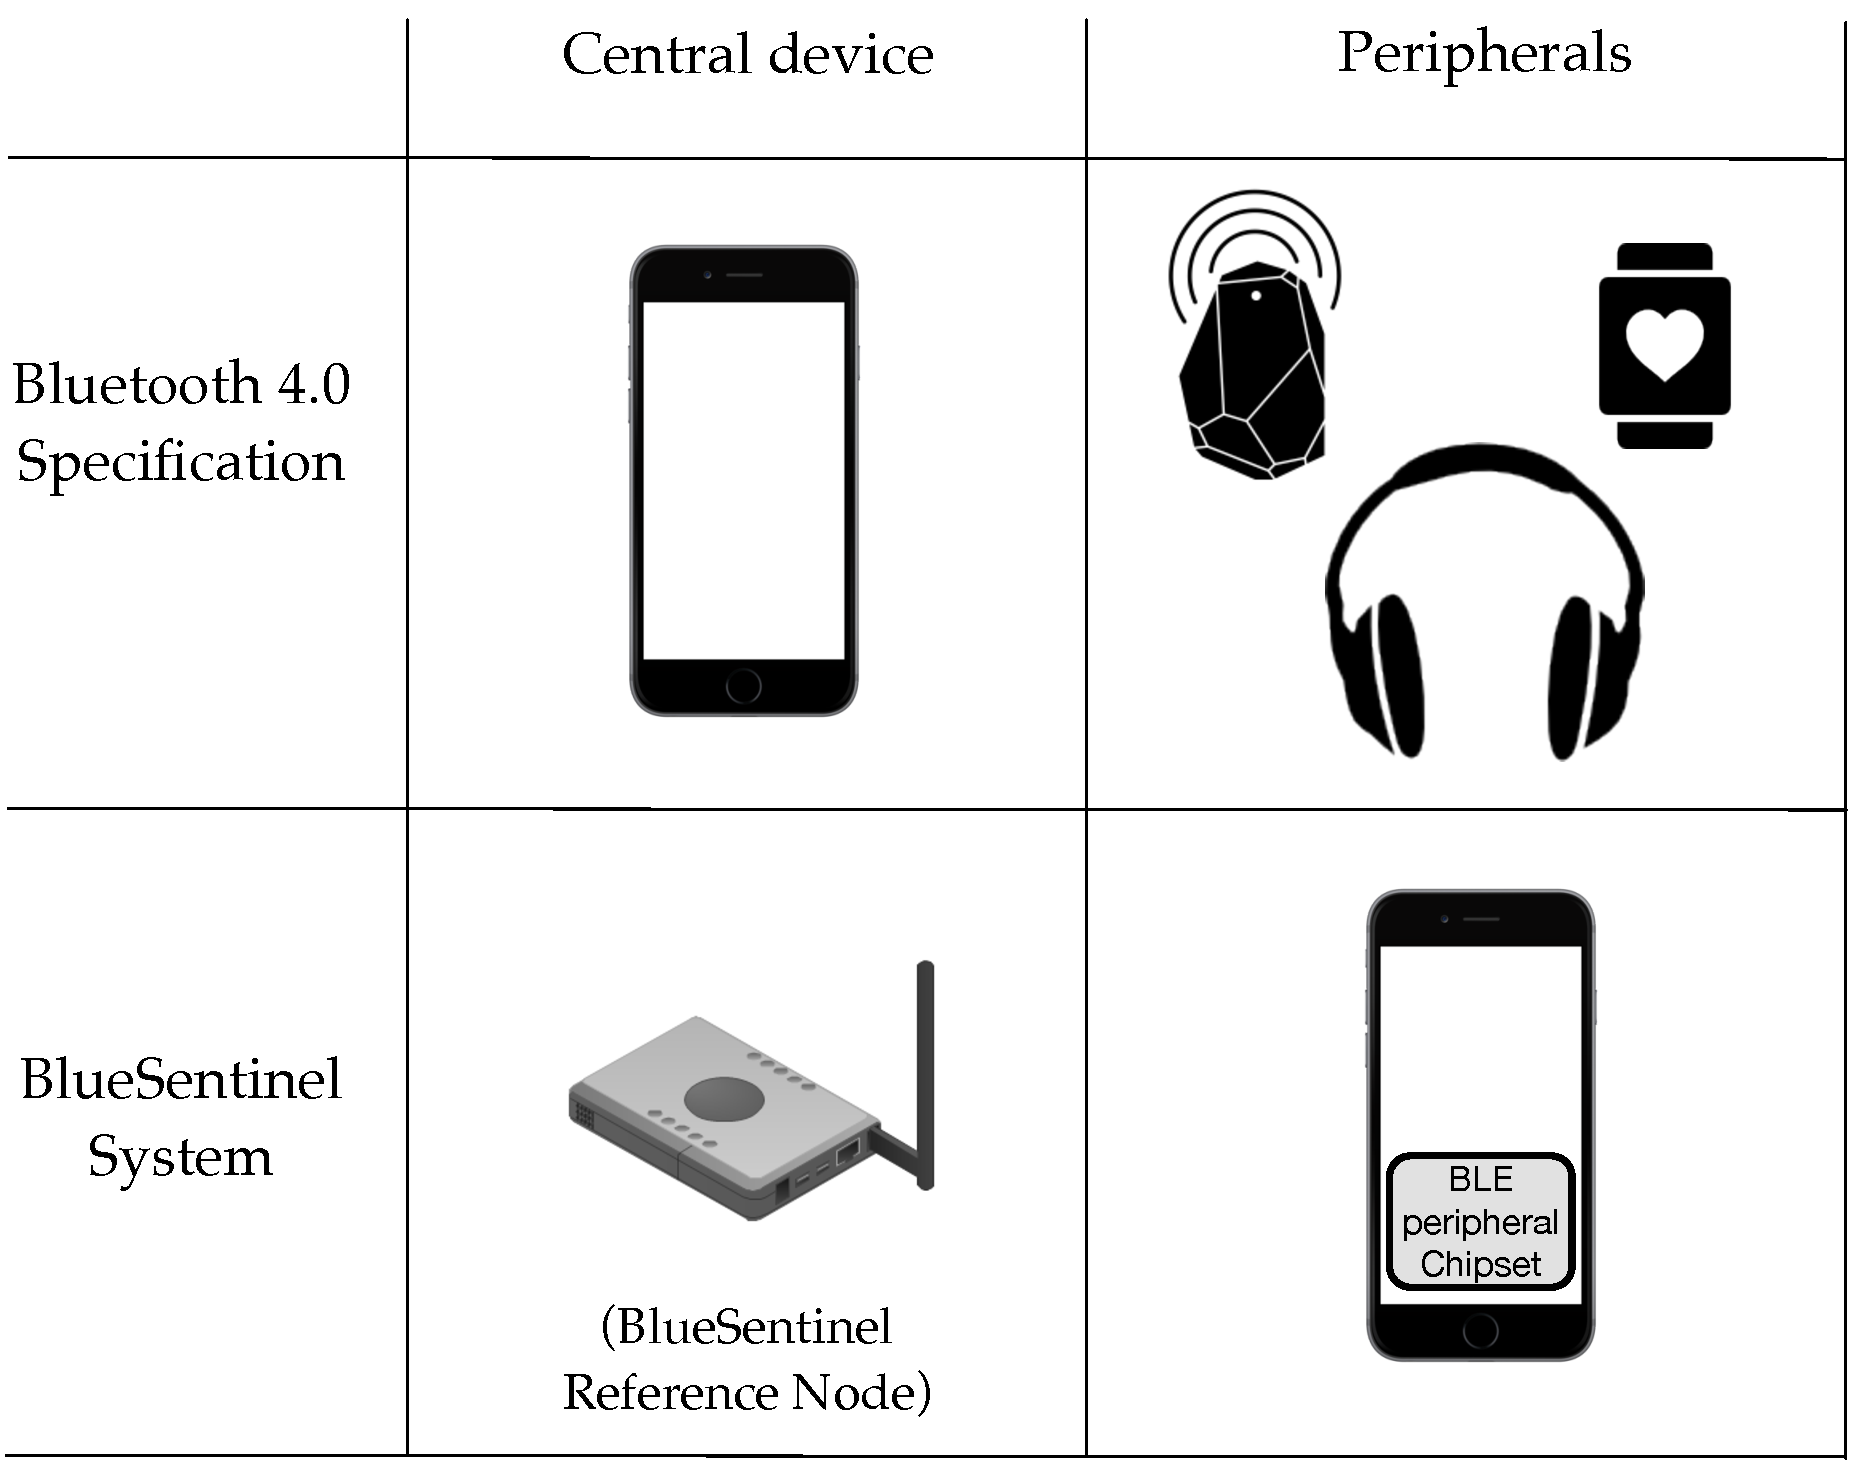
\includegraphics[width=0.8\linewidth]{central-peripheral2.pdf}
\caption[Central and Peripheral devices in BLE specification and the implemented system.]{Central and Peripheral devices in BLE specification compared with the implemented system.}
\label{fig:cent-per}
\end{figure}

The second possible way to communicate is using \emph{Advertisement}, where a BLE peripheral device broadcasts packets to every device around it. The receiving device can then act on this information.
Advertising that is by design unidirectional can be performed exclusively by peripheral devices.
For localization purposes, advertisement devices known as beacons as been employed as reference nodes; however, for localization purposes, this approach leaves the burden on the mobile device, forcing it to run positioning algorithms continuously and notify the result through energy-hungry connectivities (more details in section \ref{subsec:wips_od}).\\
The key idea behind the proposed system is to use smartphones as BLE peripheral devices, while reference nodes as BLE central devices (fig. \ref{fig:cent-per}). In this way, user devices are able to advertise them-self in a given position of the building without any connection or pairing, while reference nodes collect all the received advertisement packets.

\begin{figure}[h!tb]
\centering
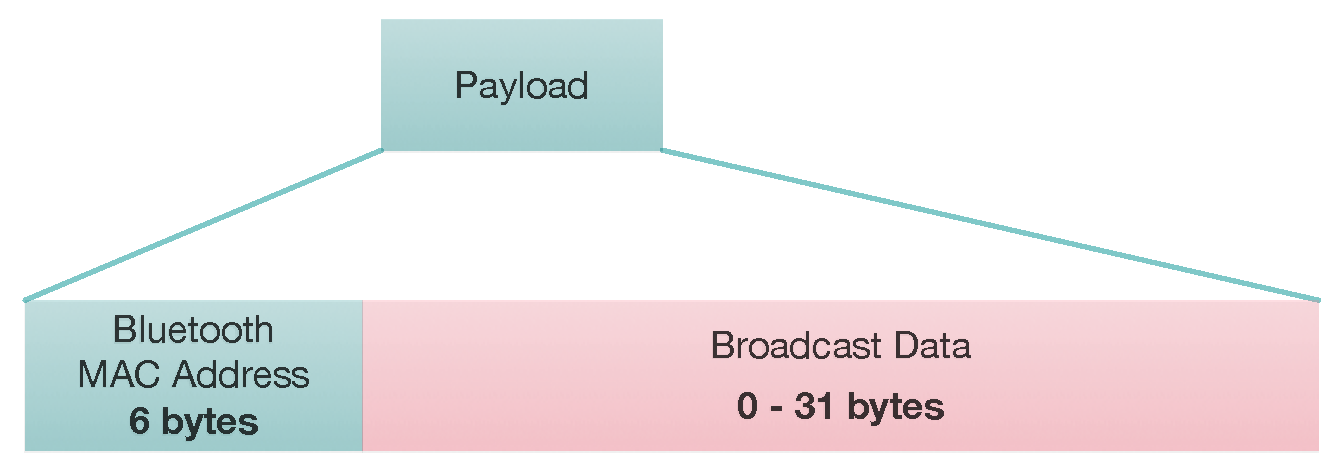
\includegraphics[width=0.65\linewidth]{payload.pdf}
\caption[BLE advertisement packet contents.]{BLE advertisement packet contents.}
\label{fig:payload}
\end{figure}

As shown in figure \ref{fig:payload}, advertisement packets contain the Bluetooth MAC address of the device and a very limited custom payload of 31 bytes. Since we need to identify the user, a straightforward solution would be to associate each MAC address with a registered user. However this is no longer possible on recent versions of Android and iOS since they hide MAC addresses to developers in order to increase user's privacy. For this reason, a Universally Unique IDentifier (UUID) has been employed to recognize each user advertisement.
At the same way in which UUIDs have been used to advertise regions through BLE beacons (like the Apple iBeacon), occupants of a building can be localized and identified in real-time associating each UUID with a building user.

BLE advertisement on mobile devices requires a specific hardware, the BLE peripheral mode chipset. Fortunately, almost all current devices have built-in peripheral chipset: all Apple devices since iPhone 4S and iPad 3, about 80\% of all Android devices released in 2014 and about 90\% in 2015 \cite{RadiusNetwork2016}.
%A Central device can't send any data to the Peripheral device without a connection. But a single peripheral can advertise to multiple masters in the area.

The proposed system has been developed using smartphones as advertising devices. However, The same advertising task can be easily implemented on wearable devices like smart-watch, that are natively build as BLE peripheral devices. The employment of wearable devices for occupancy monitoring would be even more effective, since they never separate from their users.

\section{System overview}
\label{sec:overview}
In this section, the architecture of the proposed system will be over-viewed, while in the next three sections every components will be explained in detail.

The proposed location monitoring system is composed by three main parts (figure \ref{fig:bs-protocol}).

\begin{figure}[h!tb]
\centering
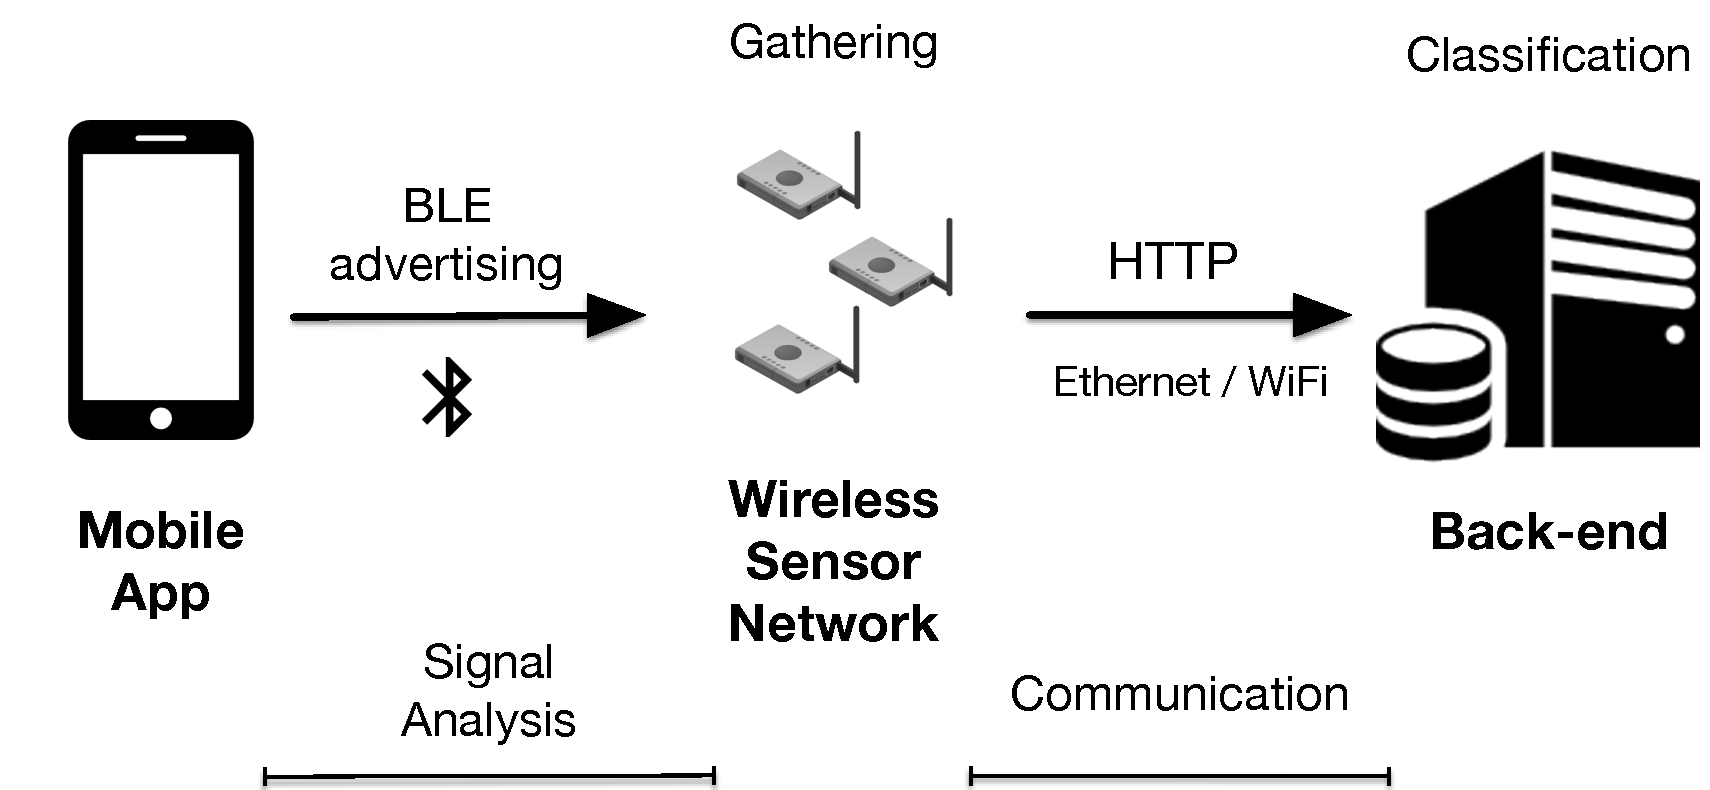
\includegraphics[width=\linewidth]{bs-protocol.pdf}
\caption[Overview of the BlueSentinel occupancy monitoring system.]{Overview of the BlueSentinel occupancy monitoring system. A mobile application perform advertising over BLE. Packets are collected by a network of sensor nodes and analyzed by a centralized system.}
\label{fig:bs-protocol}
\end{figure}

\begin{itemize}
\item First, the \textbf{mobile application} that runs on users mobile devices. The application manages registrations and logins of users (necessary to detect occupants identity) and performs the BLE advertisement. For both Android and iOS devices, it's possible to perform BLE advertisement even during device sleep and when the application is in background.
During BLE advertisement the application is free from any localization algorithm, Internet connection or GPS service, to preserve battery and to bother users as least as possible.

\item The component that directly interacts with occupants mobile devices is a network of Bluetooth Low Energy \textbf{receiver nodes}. This nodes, positioned by the building administrator during the system installation, are in charge of collecting BLE packets coming from occupants, together with signal features (like the received power) useful to estimate their position. The information collected by each node is rapidly forwarded through an Internet connection toward a centralized Building Management System.

\item All the information collected by the sensor nodes are merged at the back-end level by the \textbf{Building Management System} (BMS). Here signal features related to every occupant is reconstructed and compared to a database of training data to estimate their position. In particular, different classification algorithms have been implemented to locate each users in the best fitting zone or room. Real-time and historical data occupancy is then exposed by the BMS for a web-based monitoring and third-party applications through a REST API.
\end{itemize}

\begin{figure*}
\center
\minipage{0.40\textwidth}
  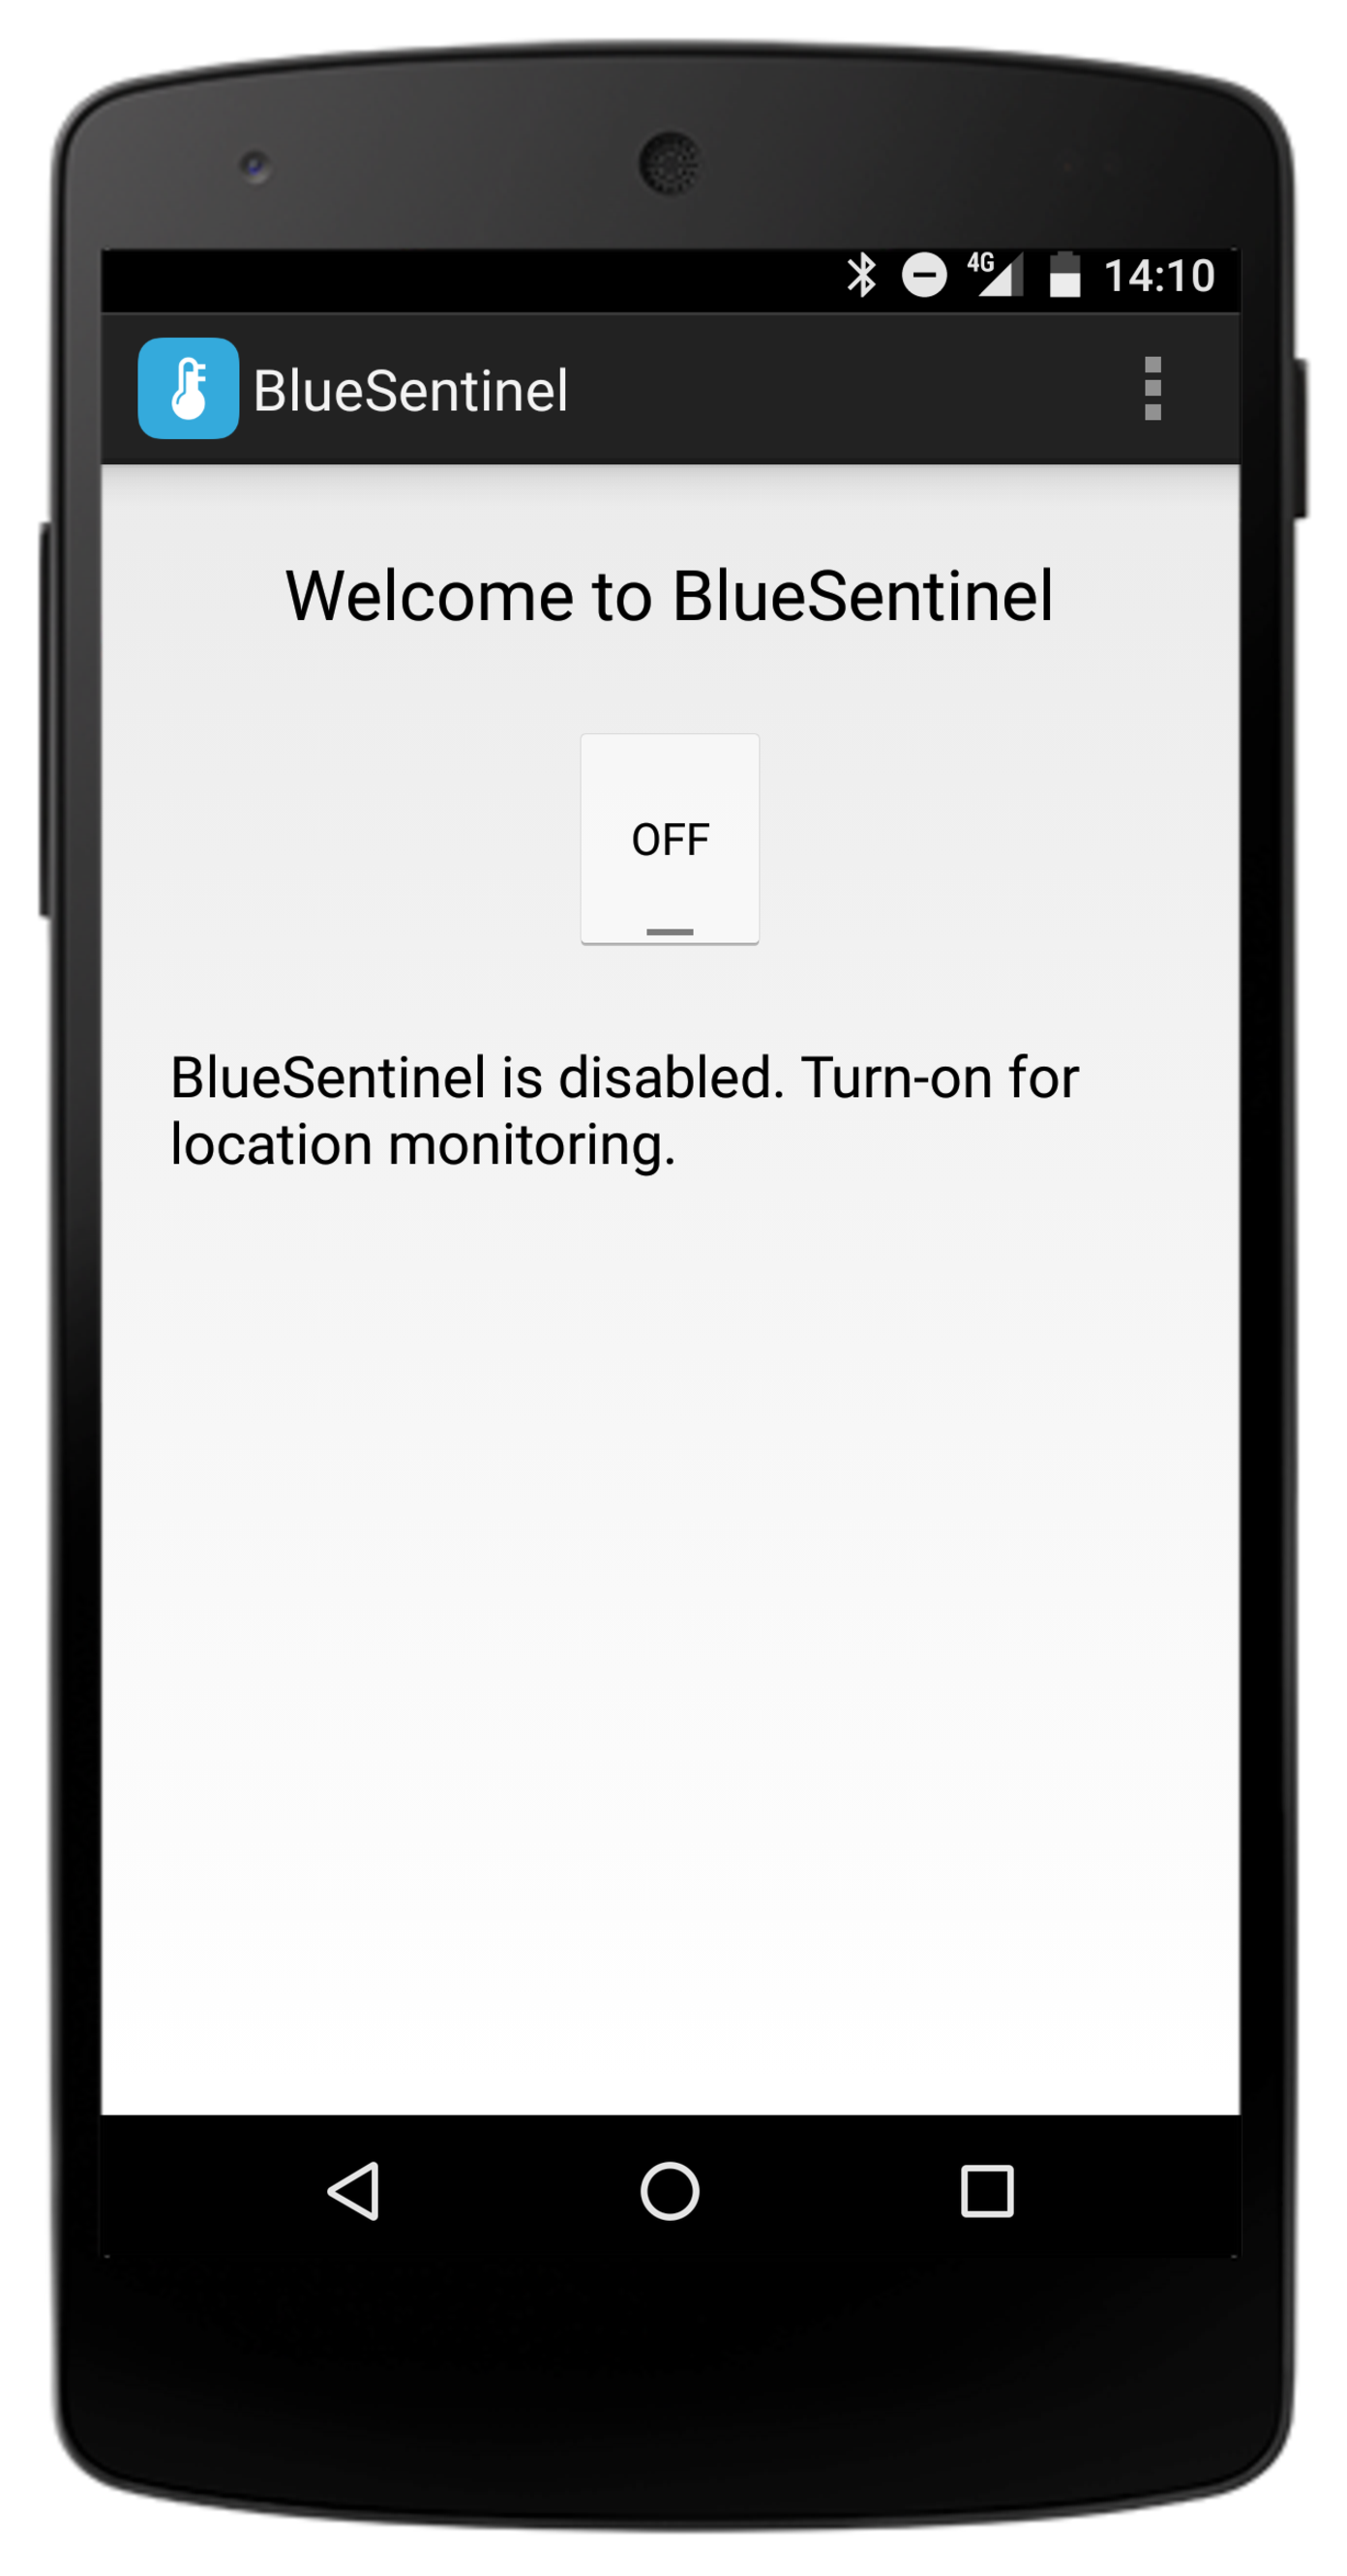
\includegraphics[width=0.85\linewidth]{bsscreen1.pdf}
\endminipage\hfill
\minipage{0.40\textwidth}%
  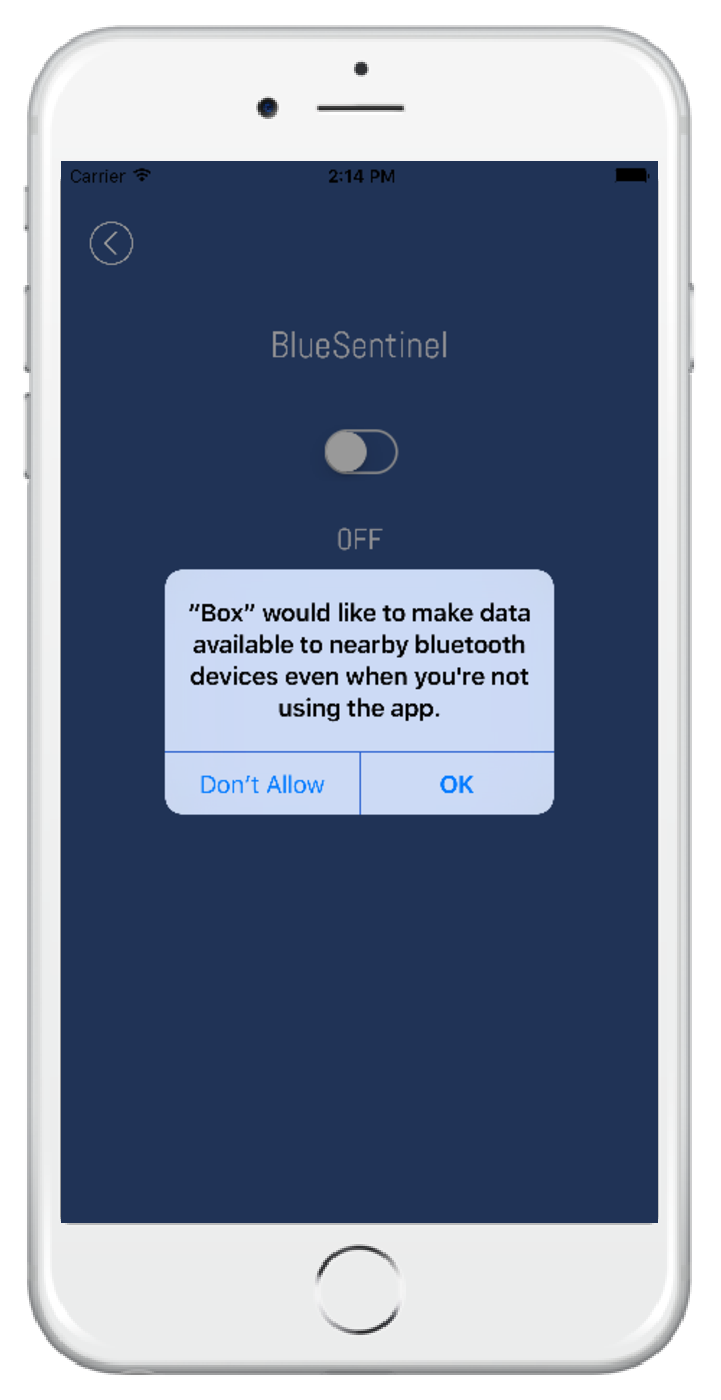
\includegraphics[width=0.85\linewidth]{bsscreen2.pdf}
\endminipage
  \caption{Mobile application developed for Android and iOS devices.}\label{fig:bsscreen}
\end{figure*}

\section{Mobile Application}
\label{sec:app}
A mobile application for both Android and iOS devices has been developed for BlueSentinel users and released on the respective store \cite{NECSTboxAndroid, NECSTboxIos} (Figure \ref{fig:bsscreen}).

The application manages users registrations to the system, asking for e-mail, username and password. Registration has been set up as mandatory; in this way the system is enabled for user identification, but also to build historical data and occupancy probability profiles per single occupant.\\
For each registered user, the system generates an identification string of 10 characters (for example \verb|userId=tslJp2hnqf|). This identifier will be used for both database key and advertisement UUID (Universally Unique IDentifier).

\lstset{
  basicstyle=\ttfamily\footnotesize,
  language=Java,
  columns=fullflexible,
  keepspaces=true,
}

The BlueSentinel menu let the user manage the Bluetooth functionality. Here BLE advertisement can be turn on and off.
In the Android environment BLE advertisement in background is supported by simply implementing the \verb|BluetoothLeAdvertiser| class in an Android Service. The essential code for the advertisement is reported in listing \ref{lst:androidAdv}.

\begin{minipage}{\linewidth}
\begin{lstlisting}[caption={BLE advertising of user identification for Android devices.}, label={lst:androidAdv}]
    private void startAdvertising() {
    		// Retrieve user identification string from database
        String userId = ParseUser.getCurrentUser().getObjectId();
        ParcelUuid pUuid = new ParcelUuid(UUID.fromString(UuidFromString("BLSNTL" + userId)));

        bleAdvertiser = BluetoothAdapter.getDefaultAdapter().getBluetoothLeAdvertiser();
        AdvertiseSettings settings = new AdvertiseSettings.Builder()
        				// Balanced transmission frequency
                .setAdvertiseMode(AdvertiseSettings.MODE_BALANCED)
                // High transmission power
                .setTxPowerLevel(AdvertiseSettings.TX_POWER_HIGH)
                // No time limit
                .setTimeout(0)
                .setConnectable(false)

        AdvertiseData data = new AdvertiseData.Builder()
        		.addServiceUuid(pUuid)
                .setIncludeDeviceName(false)
        bleAdvertiser.startAdvertising(settings, data, advCallback);
    }
\end{lstlisting}
\end{minipage}

User identification string is retrieved from database, converted into a 128-bit UUID and added to the advertisement data. An identification token ("\verb|BLSNTL|") is used as prefix in the UUID; the purpose of the prefix is to discriminate BlueSentinel UUIDs from packets advertised by unrelated devices in the environment, such as BLE headphones or wristbands. Considering 6 chars for the prefix, and the 10 chars of the id, the string of 16 characters can be contained in the 16 bytes of the UUID using the 8-bit ASCII encoding. The resulting Bluetooth packet is represented in figure \ref{fig:payload-detail}.

\begin{figure}[h!tb]
\centering
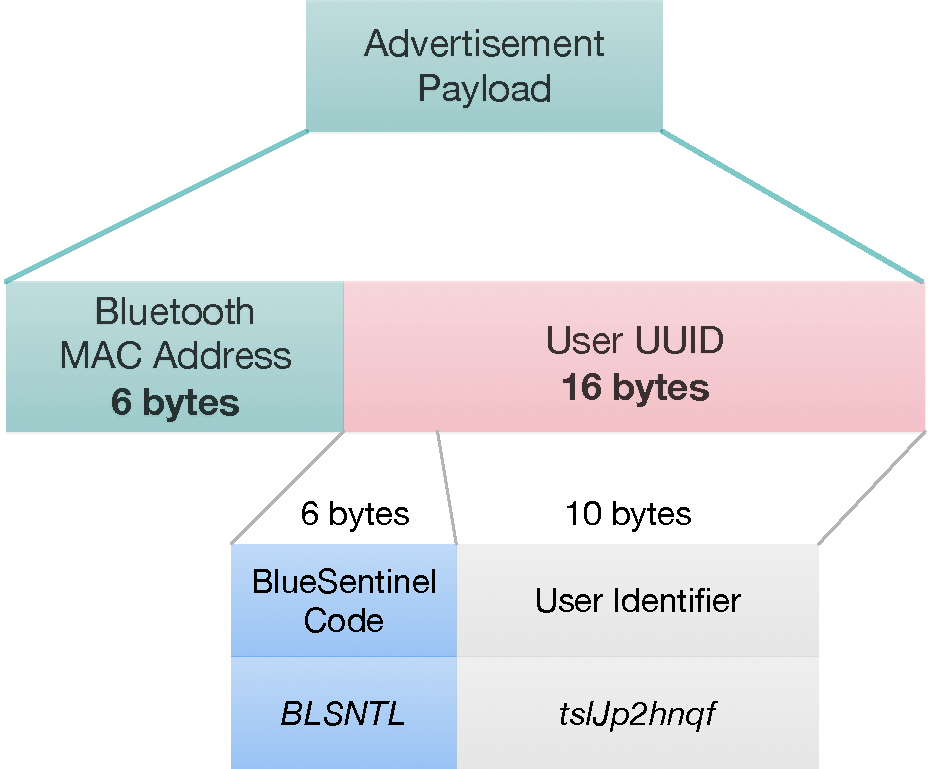
\includegraphics[width=0.6\linewidth]{payload-detail.pdf}
\caption[Detail of the BLE packet advertised by each BlueSentinel user.]{Detail of the BLE packet advertised by each BlueSentinel user.}
\label{fig:payload-detail}
\end{figure}

\medskip
In iOS SDK beacon functionalities are implemented in the CoreLocation framework, which supports all that it is needed to replicate beacons through an iDevice.
However, the CoreLocation framework places many limits on how it can be used in the background.\\
The application has been implemented exploiting the CoreBluetooth framework, that has much greater background support of iOS apps. With CoreBluetooth, it's possible to broadcast as a peripheral and detect as a central while in the background. The Objective-C code that performs the advertising is similar to the equivalent \ref{lst:androidAdv}, where the \verb|CBPeripheralManager| take the place of the \verb|BluetoothLeAdvertiser| class.


\medskip
In addition to the application for building users, a separate application has been developed for the building administrator in order to perform the training of the classification algorithm. The training requires the creation of a label for each building zone; then the administrator needs to travel across each building zone, stop for some seconds and declare the correct room label. Meanwhile, on the server side, the training phase creates a set of RSS samples, each one of them labeled with the corresponding ground truth location.

\section{Wireless Sensor Network}
\label{sec:network}
On the building side, the system requires a set of hardware nodes deployed in the indoor environment able to collect BLE packets and contact a centralized server. The node prototype has been developed using Raspberry Pi 3, one of the most cheapest board that supports all the necessary connections. In particular, the mentioned single-board computer provide a BLE module, and both WiFi and Ethernet for Internet connections.

\begin{figure}[h!tb]
\centering
\includegraphics[width=0.6\linewidth]{raspberry.png}
\caption[Prototype of BlueSentinel sensor nodes using Raspberry Pi 3 boards.]{Prototype of BlueSentinel sensor nodes using Raspberry Pi 3 boards.}
\label{fig:raspberry}
\end{figure}

Raspberry boards support a Debian-based Linux distribution, that has been used for the BlueSentinel nodes. The routine that runs continuously on each board has been written in Python, since the most supported library to manage BLE connections is provided for that language. The routine is divided in three concurrent threads:

\begin{itemize}
\item \textbf{BLE scan}: a thread is in charge of collecting every single BLE advertising signal coming from BlueSentinel users. Received packets are first filtered, searching for the BlueSentinel token inside the packet payload. All the unidentified signals are discarded, while the useful packets are stored in a queue. In particular, for each BlueSentinel packet, the thread stores the user Id, the corresponding Received Signal Strength (RSS) expressed in dBm (Decibel-milliwatt), and a timestamp representing the receiving instant.
\item \textbf{Filtering}: Like any other indoor radio-frequency signal, BLE advertisement suffer from signal fluctuations due to multipath fading. This cause a signal to fluctuate over time even if the transmitter is stationary at a fixed distance from the receiver. To reduce the error caused by fluctuations a low-pass filter is applied to the signal received by each user. The filter implemented is the Exponentially Weighted Moving Average (EWMA) that applies weighting factors to the RSS which decrease exponentially over time. Since any filter applied to smooth the signal will always introduce a delay, the EWMA filter has been selected to prioritize more recent RSS samples. The value $V_t$ is computed at time instant $t$ with the following equation:

\begin{equation}\label{eq:filter}
V_t = \alpha \cdot RSS_t + (1 - \alpha) \cdot RSS_{t-1}
\end{equation}

The weighting for each older datum decreases exponentially, never reaching zero. The $\alpha$ coefficient has been fixed to 0.75.
\item \textbf{Data push}: the third thread is is in charge of pushing RSS values periodically to the server at regular intervals. In particular, in each cycle and for each user detected, this thread send the user id, the filtered RSS values, and the most recent timestamp within the sliding window of the EWMA filter.
The choice of the timestamp is given by the weighting factor that emphasizes exponentially the more recent sample. The server is contacted with a HTTP request.
After that data is pushed to the server, the thread empty the samples queue, so that new signals coming from BLE scan will be evaluated in a new filtering window.
After some attempts with different intervals, the period has been set to 1.5 seconds.
\end{itemize}

Every nodes has been connected to the building LAN infrastructure and set up to be remotely accessed using SSH. Every relevant operation executed by the mentioned threads has been logged in a file, in order to check 

\section{Back-end}
\label{sec:back-end}
The system back-end has been set up using Parse-Server, an open-source API server based on the Express web application framework. The REST API has been exploited to interact with Parse Server from the mobile applications, sensor nodes, and a web page. The JavaScript SDK provided by Parse Server (called Cloud Code) has been used to manage the creation of database objects and the localization algorithm. The system back-end has been structured to provide the building occupancy information through the REST API to any third party components of the Building Management System able to send HTTP requests.

\begin{figure}[h!tb]
\centering
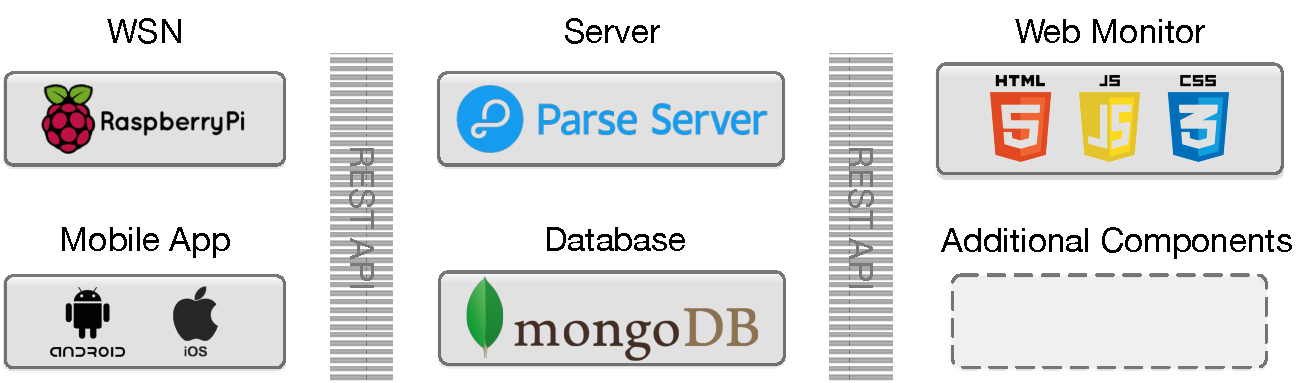
\includegraphics[width=0.9\linewidth]{platforms.pdf}
\caption[Platforms employed for the system back-end and the external components.]{Platforms employed for the system back-end and the external components.}
\label{fig:platforms}
\end{figure}

\subsection{Database}
\label{subsec:db}

The database that supports the system has been implemented using MongoDB. The database contains user objects created during registration. Each zone (or room) of the building has its own instance, created during the training phase by the administrator application. The ReceivedSignal object is created directly by the sensor nodes. It represents the reception of a BLE signal, by a given node. The object is created with the user id founded in the signal, and the received signal strength. The ReceivedSignal data is used by the fingerprinting algorithm to compute each user position. Whenever this happens, the outcome is stored using the UserPosition object.

\begin{table}
\caption{BlueSentinel back-end database}
\label{multiprogram}
\begin{tabular}{c | c c c c c}
%\cline{2-9}
Table & \multicolumn{5}{c}{Fields} \\
\hline
\multicolumn{1}{c|}{User} & userId & email & username & hashedPwd & createdAt\\
\multicolumn{1}{c|}{Zone} & \underline{zoneId} & floor & maxCapacity & label & createdAt\\
\multicolumn{1}{c|}{Node} & \underline{nodeId} & zoneId & floor & label & createdAt\\
\multicolumn{1}{c|}{ReceivedSignal} & \underline{userId} & \underline{nodeId} & RSS & \underline{timestamp} & createdAt\\
\multicolumn{1}{c|}{UserPosition} & \underline{positionId} & \underline{userId} & RSS & \underline{timestamp} & createdAt\\
\multicolumn{1}{c|}{TrainingSet} & zoneId & RSS[~] & timestamp[~] & createdAt\\
\hline
\end{tabular}
\end{table}


\subsection{Fingerprinting Algorithms}
\label{subsec:algorithms}

\section{Integration with a Thermal Comfort System}
\label{sec:thermosense}

\section{Real-World Deployed System}
\label{sec:lab}

\section{Web-Based Monitoring Dashboard}
\label{sec:webmonitor}

\section{implementation Decisions}
\label{sec:decisions}
\section{Limitations}
\label{sec:limitations}

%
% -----------------------------END------------------------------------- %